\chapter{Background and Literature Review}

This chapter surveys the research at the intersection of large language models, competitive programming, and automated test generation. It reviews existing evaluation benchmarks, targeted fault-exposure work, and bug classification systems, and ends with a gap analysis that identifies the specific limitations AlgoBugs addresses.

\section{Introduction}

Evaluation benchmarks shape how researchers understand LLM capabilities. As these models are deployed for code completion, bug detection, and test generation, the question of which capabilities they actually possess becomes important. HumanEval \cite{chen2021evaluating} asked whether a model could generate correct Python functions from a docstring. APPS \cite{hendrycks2021apps} asked whether it could solve competitive programming problems. TestCase-Eval \cite{yang2025testcase} asked whether it could expose a specific bug in a given program. Each step in this progression reveals a different kind of limitation.

This chapter traces that progression. It reviews LLMs in software engineering, code evaluation benchmarks, automated test case generation, bug taxonomy systems, and prompting strategies. The gap analysis at the end identifies what existing work cannot do and positions AlgoBugs as the first benchmark to address all four identified gaps simultaneously.

\section{Literature Review}

Figure~\ref{fig:benchmark_timeline} traces the progression of code evaluation benchmarks from 2021 to 2026. Each step moved closer to the fault-exposure task that AlgoBugs formalises.

\begin{figure}[h!]
\centering
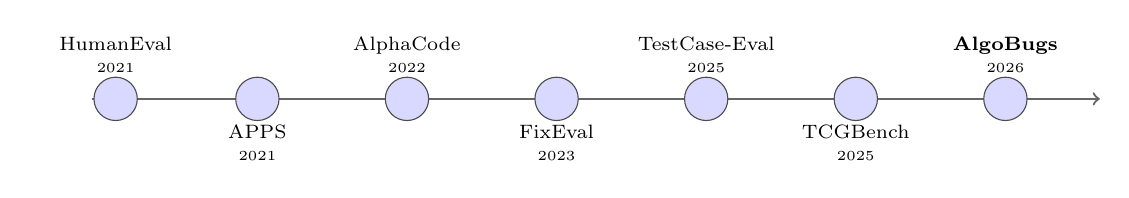
\begin{tikzpicture}[
    every node/.style={font=\small},
    ms/.style={circle, draw=black!70, fill=blue!15, minimum size=0.55cm, inner sep=0pt},
    lbl/.style={text width=2.0cm, align=center, font=\scriptsize}
]
\draw[->, thick, draw=black!60] (0,0) -- (12.8,0);
% Above: HumanEval, AlphaCode, TestCase-Eval, AlgoBugs
\foreach \x/\name/\yr in {0.3/HumanEval/2021, 4.0/AlphaCode/2022, 7.8/{TestCase-Eval}/2025, 11.6/\textbf{AlgoBugs}/2026}{
    \node[ms] at (\x,0) {};
    \node[lbl, above=6pt] at (\x,0) {\name\\{\tiny\yr}};
}
% Below: APPS, FixEval, TCGBench
\foreach \x/\name/\yr in {2.1/APPS/2021, 5.9/FixEval/2023, 9.7/TCGBench/2025}{
    \node[ms] at (\x,0) {};
    \node[lbl, below=6pt] at (\x,0) {\name\\{\tiny\yr}};
}
\end{tikzpicture}
\caption{Progression of LLM code evaluation benchmarks, 2021--2026. AlgoBugs is the first to combine competitive programming domain, fault exposure, bug taxonomy, per-category results, and execution-based evaluation.}
\label{fig:benchmark_timeline}
\end{figure}

\subsection{Large Language Models in Software Engineering}

The evaluation landscape for code-generating LLMs began with Codex \cite{chen2021evaluating}, which showed that a transformer pre-trained on GitHub code could pass roughly a third of 164 hand-written Python problems. That benchmark, called HumanEval, established pass@k as the standard metric. The problems in HumanEval were mostly library-level tasks; a model familiar with common Python idioms could score well without genuine algorithmic reasoning. This ceiling became visible quickly as models improved.

Code-specialist models such as DeepSeek-Coder \cite{guo2024deepseek} demonstrated that training specifically on code repositories yields substantially stronger performance on complex tasks. As these specialists improved rapidly, the gap between benchmark score and actual capability became harder to interpret. A model scoring 80\% on HumanEval may still fail systematically on edge cases, integer overflow, or multi-test-case state management, none of which HumanEval probes.

Huang et al.\ \cite{huang2024competition} argued that competition-level programming problems are among the most effective ways to evaluate genuine reasoning, because they cannot be solved by pattern retrieval alone. Their analysis points directly toward the evaluation setting that AlgoBugs uses: Codeforces problems, where the adversarial test culture of competitive programming forces solutions to be genuinely correct.

\subsection{Code Generation and Evaluation Benchmarks}

\textbf{Function-level benchmarks.} HumanEval \cite{chen2021evaluating} and MBPP established pass@k as the standard measure of code generation quality. Both evaluate synthesis from natural-language descriptions rather than bug detection, and both rely on static test suites. A key limitation emerged when EvalPlus extended HumanEval with LLM-generated edge cases: many solutions passing the original tests failed on the augmented ones. This implicitly previews the central problem AlgoBugs addresses, that the quality of the test cases determines what a benchmark actually measures.

\textbf{Competition-level benchmarks.} APPS \cite{hendrycks2021apps} introduced 10,000 competitive programming problems sorted by difficulty. AlphaCode \cite{li2022competition} trained on Codeforces submissions and reached roughly 50\% success on problems at its rating tier, a result that showed CP-level generation is tractable at scale. CodeContests+ \cite{wang2025codecontests} later focused specifically on test case quality for judging correctness, arguing that generating fault-exposing test inputs is a distinct and difficult challenge from generating correct code.

Despite this progression, all competition-level benchmarks retain a binary evaluation model: a submission either passes all tests or it does not. When a model fails, no information is provided about why. AlgoBugs addresses this directly by associating every submission pair with a bug category.

\textbf{Robustness.} Wang et al.\ \cite{wang2025robustness} found that LLM-generated code often passes standard tests but fails on adversarial inputs targeting specific numerical or structural assumptions. This robustness gap is precisely what AlgoBugs quantifies: the mismatch between apparent competence on aggregate benchmarks and actual ability to handle targeted, category-specific failures.

\subsection{Automated Test Case Generation and Targeted Fault Exposure}

\textbf{Traditional approaches.} Automated test generation has a long history in software engineering, spanning random testing (fuzzing), coverage-guided generation, and symbolic execution. These techniques aim to maximise structural coverage of the program under test. For competitive programming, the goal is different: not coverage maximisation but fault exposure, meaning finding a single input that demonstrates a specific existing bug. This adversarial, targeted framing is qualitatively different from traditional test generation.

\textbf{LLM-based test generation.} TestEval \cite{wang2025testeval} benchmarked LLMs on test case generation for general programming tasks, measuring fault coverage across a varied problem set. Valid test inputs could be generated across many programs, but with high variance across problem types. TestEval itself could not fully explain this variance because it reported an aggregate success rate.

\textbf{Targeted fault exposure.} TestCase-Eval \cite{yang2025testcase} and TCGBench \cite{cao2025tcgbench} are the closest prior work to AlgoBugs. In both, an LLM receives a problem description and a specific buggy solution and must generate a test input that causes the buggy solution to fail. TestCase-Eval found that even frontier models expose faults on fewer than half the pairs they are given. Both benchmarks report this as a single aggregate number. A model achieving 30\% on TestCase-Eval may succeed almost entirely on one bug category while failing completely on another; this distinction is invisible in the results.

\textbf{Execution-based evaluation.} FixEval \cite{haque2023fixeval} introduced execution-based evaluation for program repair in competitive programming, where a proposed fix is validated by running it against a test suite rather than comparing it symbolically. AlgoBugs adopts this philosophy for test generation evaluation: a generated test case is counted as successful only if the buggy solution, when executed on that input, produces a different output from the correct solution.

\subsection{Bug Taxonomy and Classification Systems}

\textbf{Production software taxonomies.} Defects4J \cite{just2014defects4j} provides 835 real-world bugs from open-source Java projects and is the standard benchmark for controlled fault studies in Java. Defects4J bugs include concurrency issues, API misuse, and framework-specific errors. These categories do not map naturally to competitive programming, where problems are single-threaded, self-contained, and time-limited.

\textbf{Competitive programming taxonomies.} Codeflaws \cite{tan2017codeflaws} introduced a taxonomy of 11 bug categories derived from competitive programming submissions in C, organised by syntactic transformation type: variable substitution, operator replacement, and similar mutations. The limitation is that syntactic transformation type does not capture the reasoning required to expose the bug. A wrong comparison operator ($>$ instead of $\geq$) and a loop boundary placed one step too low are both operator substitutions in Codeflaws, but they need qualitatively different test inputs to trigger them.

The DebugBench taxonomy provides 18 fine-grained categories for LLM debugging evaluation. That granularity produces fewer than 60 samples per class in a 1,000-pair dataset, which is too sparse for statistically reliable per-category analysis. At the other extreme, a three-to-five category taxonomy would subsume qualitatively different bugs under single labels, reducing diagnostic value.

\textbf{The AlgoBugs taxonomy design.} The AlgoBugs taxonomy occupies the middle ground: eight categories, mutually exclusive and covering the main failure modes in C++ competitive programming, with approximately 125 samples per class in the 1,000-pair dataset. The full taxonomy definition is in Chapter~3.

\subsection{Prompting Strategies for Code-Related Reasoning}

\textbf{Zero-shot prompting} presents the model with a task description and input without any worked examples \cite{learnprompting2025shot}. In the AlgoBugs setting, the model receives the problem statement and buggy code and is asked to generate a fault-exposing test case directly. This measures the model's baseline fault-exposure capability without cognitive scaffolding.

\textbf{Chain-of-thought prompting} instructs the model to produce intermediate reasoning steps before its final answer \cite{wei2022chain}. Li et al.\ \cite{li2025uncertainty} extended this to code generation with uncertainty-guided CoT, finding that explicit reasoning steps improve correctness on multi-step logical problems. For fault exposure, CoT asks the model to first identify the logical flaw, then design a test that triggers it. Whether this structured approach improves performance depends on the bug category, which is one of the questions AlgoBugs tests directly.

\textbf{Few-shot prompting} augments the prompt with labelled examples \cite{promptpanda2025few}. AlgoBugs evaluates few-shot prompting using three synthetic task-level demonstrations, one each for a representative T1 (integer overflow), T3 (off-by-one), and T4 (wrong conditional) bug. Unlike category-matched examples drawn from the dataset itself, synthetic demonstrations teach the fault-targeting reasoning pattern without risking data leakage. This design isolates whether task-format examples alone can improve FER, independent of category-specific grounding. Zero NO\_TEST\_GENERATED failures were observed under few-shot prompting, compared to rates of 1--29\% under chain-of-thought, showing that worked examples also anchor the required output format.

\begin{table}[h!]
\centering
\caption{Summary of Literature Reviewed.}
\label{tab:lit_review}
\renewcommand{\arraystretch}{1.3}
\resizebox{\linewidth}{!}{%
\begin{tabular}{|p{2.5cm}|c|p{3.5cm}|p{3.5cm}|p{4.5cm}|}
\hline
\textbf{Author(s)} & \textbf{Year} & \textbf{Title} & \textbf{Methodology} & \textbf{Key Findings} \\
\hline
Chen et al.\ \cite{chen2021evaluating} & 2021 & Evaluating LLMs trained on code & Transformer pre-trained on GitHub code & Introduced HumanEval and pass@k; showed LLMs can solve function-level programming tasks. \\
\hline
Guo et al.\ \cite{guo2024deepseek} & 2024 & DeepSeek-Coder & Code-specialist LLM training on code repos & Code-specific training yields substantially better performance than general-purpose LLMs on complex tasks. \\
\hline
Huang et al.\ \cite{huang2024competition} & 2024 & Competition-level problems as LLM evaluators & Analysis of CP as evaluation setting & CP problems reveal reasoning limits that simpler benchmarks miss. \\
\hline
Hendrycks et al.\ \cite{hendrycks2021apps} & 2021 & Measuring coding challenge competence with APPS & 10,000 CP problems, pass@k evaluation & Competition-level evaluation exposes limits that are invisible in function-level benchmarks. \\
\hline
Li et al.\ \cite{li2022competition} & 2022 & Competition-level code generation with AlphaCode & Large-scale CP generation model & Achieved approximately 50\% success at its rating tier; showed CP generation is tractable at scale. \\
\hline
Wang et al.\ \cite{wang2025codecontests} & 2025 & CodeContests+: high-quality test case generation & Test case quality analysis for CP & Test case quality is a distinct and difficult challenge separate from code generation. \\
\hline
Wang et al.\ \cite{wang2025robustness} & 2025 & Empirical study on robustness of LLM code & Adversarial input analysis & LLM-generated code often passes standard tests but fails on adversarial edge-case inputs. \\
\hline
Wang et al.\ \cite{wang2025testeval} & 2025 & TestEval: benchmarking LLMs for test case generation & LLM evaluation on test generation & Valid tests can be generated broadly, but with high variance across problem types. \\
\hline
Yang et al.\ \cite{yang2025testcase} & 2025 & TestCase-Eval: fault coverage and exposure & Targeted fault-exposure evaluation & Frontier models expose fewer than 50\% of faults; task is genuinely difficult for current LLMs. \\
\hline
Cao et al.\ \cite{cao2025tcgbench} & 2025 & TCGBench: test case generation for CP & Evaluation on competition-level problems & Corroborates TestCase-Eval findings; models struggle with adversarial fault-exposing inputs. \\
\hline
Haque et al.\ \cite{haque2023fixeval} & 2023 & FixEval: execution-based evaluation for CP fixes & Execution-based evaluation methodology & Execution-based validation is more reliable than syntactic comparison for correctness assessment. \\
\hline
Just et al.\ \cite{just2014defects4j} & 2014 & Defects4J: a database of existing Java faults & Controlled Java fault database & Gold standard for Java fault studies; categories do not map to CP algorithmic failures. \\
\hline
Tan et al.\ \cite{tan2017codeflaws} & 2017 & Codeflaws: a CP benchmark for program repair & 11-category syntactic mutation taxonomy & Classifies CP bugs by syntactic transformation type, not by the reasoning required to expose them. \\
\hline
\end{tabular}%
}
\end{table}

\section{Gap Analysis}

Figure~\ref{fig:venn_positioning} positions AlgoBugs within the landscape of related research by identifying the three research areas whose intersection it occupies.

\begin{figure}[h!]
\centering
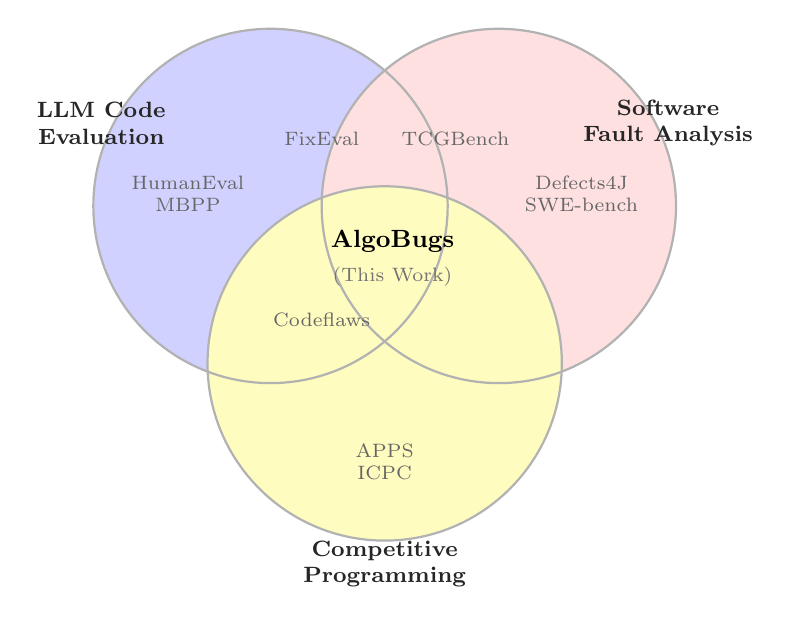
\begin{tikzpicture}[font=\small]
    \fill[blue!18]  (-1.45, 0.85) circle (2.25cm);
    \fill[red!12]   ( 1.45, 0.85) circle (2.25cm);
    \fill[yellow!25]( 0.00,-1.15) circle (2.25cm);

    \draw[gray!60, thick] (-1.45, 0.85) circle (2.25cm);
    \draw[gray!60, thick] ( 1.45, 0.85) circle (2.25cm);
    \draw[gray!60, thick] ( 0.00,-1.15) circle (2.25cm);

    \node[font=\footnotesize\bfseries, text=black!85, align=center] at (-3.6,  1.9) {LLM Code\\Evaluation};
    \node[font=\footnotesize\bfseries, text=black!85, align=center] at ( 3.6,  1.9) {Software\\Fault Analysis};
    \node[font=\footnotesize\bfseries, text=black!85, align=center] at ( 0.0, -3.7) {Competitive\\Programming};

    \node[font=\scriptsize, text=black!60, align=center] at (-2.5,  1.0) {HumanEval\\MBPP};
    \node[font=\scriptsize, text=black!60, align=center] at ( 2.5,  1.0) {Defects4J\\SWE-bench};
    \node[font=\scriptsize, text=black!60, align=center] at ( 0.0, -2.4) {APPS\\ICPC};

    \node[font=\scriptsize, text=black!60, align=center] at (-0.8,  1.7) {FixEval};
    \node[font=\scriptsize, text=black!60, align=center] at ( 0.9,  1.7) {TCGBench};
    \node[font=\scriptsize, text=black!60, align=center] at (-0.8, -0.6) {Codeflaws};

    \node[font=\small\bfseries, text=black, align=center] at ( 0.1,  0.4) {\textbf{AlgoBugs}};
    \node[font=\scriptsize, text=black!55, align=center] at ( 0.1, -0.05) {(This Work)};
\end{tikzpicture}
\caption{Research positioning of AlgoBugs. It is the first benchmark at the intersection of LLM code evaluation, software fault analysis, and competitive programming. Existing work addresses at most two dimensions simultaneously: TCGBench covers fault exposure and competitive programming but lacks a bug taxonomy; FixEval evaluates LLM fault exposure but outside the competitive programming domain.}
\label{fig:venn_positioning}
\end{figure}

Table~\ref{tab:gap_analysis} compares AlgoBugs against the eight most closely related benchmarks on five design criteria: whether they target the competitive programming domain, whether they evaluate fault exposure specifically, whether they include a structured bug taxonomy, whether they report per-category results, and whether they use execution-based evaluation.

\begin{table}[h!]
\centering
\caption{Comparison of existing benchmarks and their limitations relative to AlgoBugs.}
\label{tab:gap_analysis}
\renewcommand{\arraystretch}{1.3}
\resizebox{\linewidth}{!}{%
\begin{tabular}{lcccccc}
\toprule
\textbf{Benchmark} & \textbf{CP Domain} & \textbf{Fault Exposure} & \textbf{Bug Taxonomy} & \textbf{Per-Category} & \textbf{Execution-Based} \\
\midrule
HumanEval \cite{chen2021evaluating}   & $\times$ & $\times$ & $\times$ & $\times$ & \checkmark \\
APPS \cite{hendrycks2021apps}          & \checkmark & $\times$ & $\times$ & $\times$ & \checkmark \\
Codeflaws \cite{tan2017codeflaws}      & \checkmark & $\times$ & \checkmark & $\times$ & \checkmark \\
Defects4J \cite{just2014defects4j}     & $\times$ & $\times$ & \checkmark & $\times$ & \checkmark \\
FixEval \cite{haque2023fixeval}        & \checkmark & \checkmark & $\times$ & $\times$ & \checkmark \\
TestEval \cite{wang2025testeval}       & $\times$ & \checkmark & $\times$ & $\times$ & \checkmark \\
TestCase-Eval \cite{yang2025testcase}  & \checkmark & \checkmark & $\times$ & $\times$ & \checkmark \\
TCGBench \cite{cao2025tcgbench}        & \checkmark & \checkmark & $\times$ & $\times$ & \checkmark \\
\midrule
\textbf{AlgoBugs (This Work)}          & \checkmark & \checkmark & \checkmark & \checkmark & \checkmark \\
\bottomrule
\end{tabular}%
}
\end{table}

The table shows that TestCase-Eval and TCGBench come closest to AlgoBugs: both target the competitive programming domain, both evaluate fault exposure, and both use execution-based evaluation. Neither, however, associates results with a structured bug taxonomy or reports per-category fault-exposure rates. AlgoBugs is the first benchmark to satisfy all five criteria simultaneously.

Four specific gaps in the existing literature motivate the AlgoBugs design:

\textbf{Gap 1: No diagnostic granularity.} All prior fault-exposure benchmarks report a single aggregate success rate. They establish that this task is difficult for current LLMs but cannot say which aspects of algorithmic reasoning drive success or failure. AlgoBugs resolves this by categorising every bug instance under the eight-category taxonomy and reporting per-category FER for each model.

\textbf{Gap 2: No semantically grounded bug taxonomy for CP.} Codeflaws classifies bugs by syntactic transformation type rather than by the cognitive failure they represent. A wrong comparison operator and an off-by-one loop bound are both operator substitutions in Codeflaws, but they demand different test inputs. AlgoBugs introduces a taxonomy designed specifically to separate the reasoning capabilities each category requires.

\textbf{Gap 3: Data contamination risk.} Many benchmarks draw from datasets that likely overlap with LLM training corpora, potentially inflating evaluation scores. AlgoBugs sources exclusively from Codeforces rounds published after January 2021 and prioritises problems with limited internet presence at the time of data collection.

\textbf{Gap 4: No cross-model diagnostic comparison.} No prior work systematically compares multiple model tiers at the category level on the same fault-exposure task. AlgoBugs provides this comparison across five models under two prompting strategies, enabling both cross-model and cross-category analysis.

\section{Summary}

The literature shows a consistent progression: code evaluation benchmarks have moved from function-level synthesis tasks toward competition-level fault exposure. Each step has increased the difficulty and realism of the evaluation. One design choice, however, has persisted throughout: aggregate, category-blind success rates.

AlgoBugs builds directly on the most advanced prior work, TestCase-Eval and TCGBench, while addressing the four gaps identified above. By structuring a 1,000-pair competitive programming dataset under an eight-category bug taxonomy and evaluating five models with both zero-shot and chain-of-thought prompting, AlgoBugs provides the first diagnostic profile of LLM fault-exposure capabilities. The result is not just a measurement of how well models perform, but a map of where their reasoning is reliable and where it consistently breaks down.
